\chapter{Prototype haute performance}
\label{chap:protoHP}

Dans un cadre d'application comme celui de la réalité augmentée spatiale ou les interactions jouent un rôle majeure dans l'expérience de l'utilisateur la réactivité, la fluidité de l'expérience et la latence générale du système sont des points cruciaux qu'il est impossible de négliger. Pour pouvoir atteindre ces objectifs et pouvoir pousser les applications encore plus loin aussi bien dans l'interaction, dans le rendu ou dans le contenu, sans avoir besoin d'une puissance de calcul dépassant l'entendement, une optimisation aussi bien logicielle, matérielle ou architecturale est nécessaire. Cette optimisation a fait l'objet d'une grande partie de mon stage qui m'a amener a développer un prototype dit "haute performance" des outils que propose \texttt{RealityTech}. L'optimisation logicielle c'est surtout porté sur l'amélioration des performances des algorithmes de traitement d'image bien connus pour être extrêmement consommateur des ressources. Pour l'optimisation matérielle, la tâche a était un peu différentes et nous nous sommes attelé à effectuer des mesures et des calculs sur la puissance théorique du matériel, la latence réel des caméra ou encore la rapidité de l'encodage des flux vidéos pour arriver à établir les performances réelles qu'il nous était possible d'atteindre avec différentes combinaison de matériel. Le développement du prototype s'est achevé avec la création d'une nouvelle architecture logiciel en micro services dans le but de créer un environnement modulaire réactif ou les services peuvent mourir sans mettre en péril tout le système et ainsi améliorer grandement la qualité général des outils fournis.

\section{Amélioration logiciel}
De nos jour, les optimisations font l'objet de développements ciblés et très spécifique, se concentrant la plupart du temps sur l'amélioration d'un unique point cruciale d'un algorithme ou d'une application. Dans notre cas l'optimisation logiciel a surtout été effectué au niveau des algorithmes de traitement d'images omniprésent et indispensable a la technologie. La réalité augmentée spatiale a besoin du monde réel pour exister c'est pourquoi le matériel dispose de nombreux capteurs (caméras) pour l'analyser et que de nombreux algorithmes de traitement des données captés (images) sont mis en place. Après une rapide analyse du logiciel, il est indéniable que traitement le plus utilisé est la convolution d'une image par un filtre qui possède un nombre incalculable d'application et c'est pourquoi nous avons choisit de concentrer nos efforts sur l'optimisation de ce dernier.

\subsection{Convolution - Théorie}
\begin{quotation}
\textit{En mathématiques, le produit de convolution est un opérateur bilinéaire et un produit commutatif, généralement noté $∗$, qui, à deux fonctions f et g sur un même domaine infini, fait correspondre une autre fonction $f * g$ sur ce domaine, qui en tout point de celui-ci est égale à l'intégrale sur l'entièreté du domaine (ou la somme si celui-ci est discret) d'une des deux fonctions autour de ce point, pondérée par l'autre fonction autour de l'origine — les deux fonctions étant parcourues en sens contraire l'une de l'autre (nécessaire pour garantir la commutativité).\footnote{Source: \href{https://fr.wikipedia.org/wiki/Produit_de_convolution}{Produit de convolution - Wikipedia}}}
\end{quotation}

Dans le cadre du traitement d'image, le produit de convolution représente une technique de filtrage d'image visant à accentuer ou atténuer certaines caractéristiques ce celle ci comme la netteté, le flou ou les zones de fort gradient (les contours) par exemple (fig ~\ref{fig:conv:filter}). Étant donné que nous travaillons avec des images définit par un nombre fini de pixels, la convolution d'une image est réalisée dans le domaine discret où $f$ et $g$ dans la définition mathématique représentent respectivement une image et le filtre qu'on souhaite lui appliquer. Le résultat de cette convolution est une nouvelle image.

On appel filtre, ou noyau de convolution, une image (ou une matrice) généralement de petite taille définit en amont qui va être utilisée pour calculer la nouvelle valeur de chacun des pixels de l'image résultat. C'est la définition de ce dernier qui va décider du traitement appliquer à l'image. 

Le calcul de la valeur d'un pixel dans l'image résultat se fait de la manière suivante : Le voisinage autour du pixel dont on souhaite calculé la valeur est pondéré par le filtre de convolution que l'on aura préalablement centré sur ce pixel. La nouvelle valeur du pixel représente la somme de toutes les valeurs précédemment calculées.

Sur la figure ~\ref{fig:conv:image} on souhaite calculer la nouvelle valeur du pixel positionné en 3,3 dans l'image d'origine (I). On sélectionne donc un voisinage de même taille que le filtre (K) centré sur ce pixel dont chaque élément va être multiplié par la valeur du filtre pour calculée la valeur du pixel 3,3 dans la nouvelle image soit 
\begin{center}
$I_{3,3} * K = 88 * 1/9 + 21 * 1/9 + 25 * 1/2 + 68 * 1/9 + 14 * 1/9 + 15 * 1/9 + 35 * 1/9 + 52 * 1/9 + 10 * 1/9 = 36$.
\end{center}

\begin{figure}[H]
\centering
	\subfloat[Image originale]{
      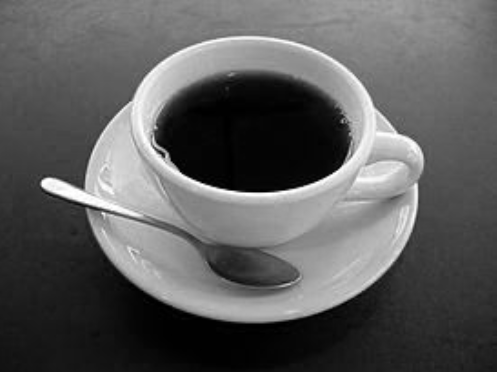
\includegraphics[width=0.33\textwidth]{images/coffee-identity}
      \label{sub:conv:filter:original}
      }
     \subfloat[Filtre contour]{
      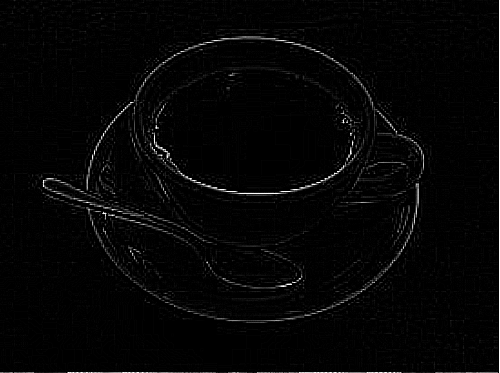
\includegraphics[width=0.33\textwidth]{images/coffee-outline}
      \label{sub:conv:filter:outline}
      }
      \\
      	\subfloat[Filtre de netteté]{
      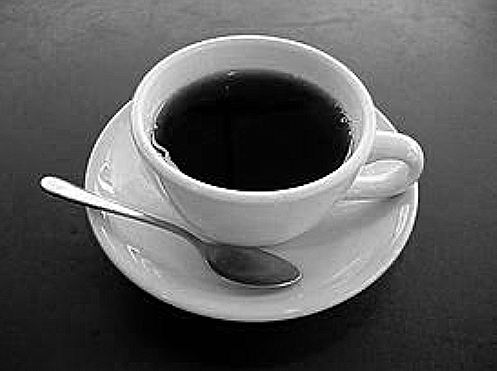
\includegraphics[width=0.33\textwidth]{images/coffee-sharpen}
      \label{sub:conv:filter:sharpen}
      }
     \subfloat[Filtre relief]{
      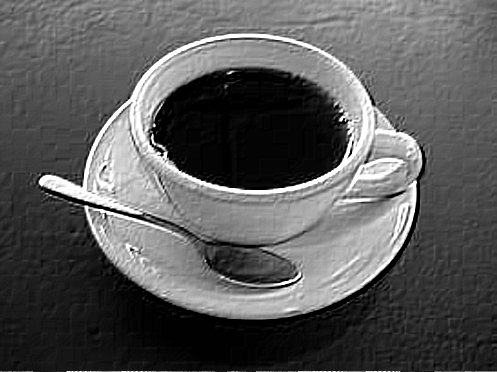
\includegraphics[width=0.33\textwidth]{images/coffee-emboss}
      \label{sub:conv:filter:emboss}
      }
\caption{Différentes filtres de convolution appliquée à une image.}
\label{fig:conv:filter}
\end{figure}

\begin{figure}[H]
\centering
\begin{tikzpicture}
	\matrix (mtr) [matrix of nodes,row sep=-\pgflinewidth, nodes={draw,  minimum size=5.7mm, anchor=center}]
	{
		12 & 46  & 05 & 94 & 25 & 00 & 87\\
		05 & 13  & 01 & 20 & 25 & 00 & 37\\
		72 & 25  & |[fill=red!30]| 88 & |[fill=red!30]| 21 & |[fill=red!30]| 25 & 00 & 99\\
		21 & 74  & |[fill=red!30]| 68 & |[fill=red!30]| 14 & |[fill=red!30]| 15 & 00 & 61\\
		48 & 97  & |[fill=red!30]| 35 & |[fill=red!30]| 52 & |[fill=red!30]| 10 & 00 & 42\\
		11 & 29  & 57 & 00 & 75 & 00 & 12\\
		17 & 01  & 78 & 00 & 50 & 00 & 12\\
		16 & 54  & 00 & 00 & 25 & 00 & 11\\
	};

	\draw[very thick, red] (mtr-3-3.north west) rectangle (mtr-5-5.south east);

	\node [below= of mtr-8-4.south] (lm) {$\bf I$};
	\node[right = 0.2em of mtr] (str) {$* \frac{1}{9}$};

	\matrix (K) [right=0.2em of str,matrix of nodes,row sep=-\pgflinewidth, nodes={draw, fill=blue!30,  minimum size=5.7mm, anchor=center}]
	{
		1 & 1 & 1 \\
		1 & 1 & 1 \\
		1 & 1 & 1 \\
	};
	\node [below = of K-3-2.south] (lk) {$\bf K$};

	\node [right = 0.2em of K] (eq) {$=$};

	\matrix (ret) [right=0.2em of eq,matrix of nodes,row sep=-\pgflinewidth, nodes={draw, minimum size=5.7mm, anchor=center}, nodes in empty cells]
	{
		 &   &  &  &  &  & \\
		 &   &  &  &  &  & \\
		 &   &  &  &  &  & \\
		 &   &  & |[fill=green!30]| 36 &  &  & \\
		 &   &  &  &  &  & \\
		 &   &  &  &  &  & \\
		 &   &  &  &  &  & \\
		 &   &  &  &  &  & \\
	};
	\node [below = of ret-8-4.south] (lim) {${\bf I_{i,j}} * {\bf K}$};

	\draw[very thick, green] (ret-4-4.north west) rectangle (ret-4-4.south east);

	\draw[densely dotted, blue, thick] (mtr-3-3.north west) -- (K-1-1.north west);
	\draw[densely dotted, blue, thick] (mtr-5-3.south west) -- (K-3-1.south west);
	\draw[densely dotted, blue, thick] (mtr-3-5.north east) -- (K-1-3.north east);
	\draw[densely dotted, blue, thick] (mtr-5-5.south east) -- (K-3-3.south east);

	\draw[densely dotted, green, thick] (ret-4-4.north west) -- (K-1-1.north west);
	\draw[densely dotted, green, thick] (ret-4-4.south west) -- (K-3-1.south west);
	\draw[densely dotted, green, thick] (ret-4-4.north east) -- (K-1-3.north east);
	\draw[densely dotted, green, thick] (ret-4-4.south east) -- (K-3-3.south east);

	\draw[very thick, blue] (K-1-1.north west) rectangle (K-3-3.south east);

	\node[anchor=south east, inner sep=0.01em, blue] at (mtr-3-3.south east) (xx) {\scalebox{.5}{$\times 1$}};
	\node[anchor=south east, inner sep=0.01em, blue] at (mtr-3-4.south east) (xx) {\scalebox{.5}{$\times 1$}};
	\node[anchor=south east, inner sep=0.01em, blue] at (mtr-3-5.south east) (xx) {\scalebox{.5}{$\times 1$}};
	\node[anchor=south east, inner sep=0.01em, blue] at (mtr-4-3.south east) (xx) {\scalebox{.5}{$\times 1$}};
	\node[anchor=south east, inner sep=0.01em, blue] at (mtr-4-4.south east) (xx) {\scalebox{.5}{$\times 1$}};
	\node[anchor=south east, inner sep=0.01em, blue] at (mtr-4-5.south east) (xx) {\scalebox{.5}{$\times 1$}};
	\node[anchor=south east, inner sep=0.01em, blue] at (mtr-5-3.south east) (xx) {\scalebox{.5}{$\times 1$}};
	\node[anchor=south east, inner sep=0.01em, blue] at (mtr-5-4.south east) (xx) {\scalebox{.5}{$\times 1$}};
	\node[anchor=south east, inner sep=0.01em, blue] at (mtr-5-5.south east) (xx) {\scalebox{.5}{$\times 1$}};
\end{tikzpicture}
\caption{Convolution d'une matrice (image) (I) par un filtre (K)}
\label{fig:conv:image}
\end{figure}

Comme on peut s'en rendre compte, l'image résultat est une nouvelle image, totalement indépendante de l'image d'origine dont chaque pixel est complètement indépendant de ces voisins. C'est cette propriété qui va nous intéressé car cela signifie qu'il est possible de calculer chaque pixel de l'image résultat dans n'importe quel ordre et qu'avec des moyens de calculs suffisant il est possible de calculer tous les pixels de l'image résultat en une seule fois. On dit d'une telle fonction qu'elle est parallélisable. Ce fort potentiel de parallélisation fait de ce traitement une cible de choix pour l'optimisation et donc le calcul sur carte graphique (section ~\ref{chap:notions} - Calcul haute performance).

\subsection{Convolution - Implémentation sur GPU}
Il existe de nos jours plusieurs langage de programmation graphique nous permettant de mettre à profit la puissance de notre GPU. Nous avons choisit d'implémenter notre algorithme de convolution dans 3 de ces langages en OpenCL %TODO cité
OpenGL ES %TODO cité
et CUDA %TODO cité
enfin d'en évaluer les compétences et d'en comparer les différentes performances.

\paragraph{OpenCL} OpenCL ou \emph{Open Computing Language} est un language de programmation basé le C créé par \texttt{Khronos Group} en 2009.
Un programme OpenCL est composé de deux partie :
La partie \textbf{code hôte} qui est l'application principale et qui va se charger d'orchestrer les différentes tâches. Cette partie est écrite en C avec des appels a l'API OpenCL pour gérer tout ce qui allocation de mémoire et gestion des périphériques OpenCL.
La partie \textbf{noyau} ou \textbf{code périphérique} qui représente un programmes qui va être exécutés sur un périphérique. Cette partie est écrite en OpenCL-C et représente les calculs à effectuer.
Il faut aussi bien différencier hôte, qui dans notre cas sera le processeur et qui sert a allouer la mémoire et transférer les données au périphérique, et périphérique(s) qui représentera ici une ou plusieurs carte graphique et qui sera utilisé appliquer des traitements aux données qui lui sont transmise.
\begin{figure}[H]
\centering
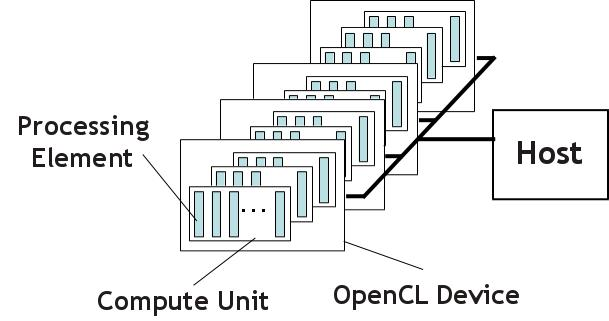
\includegraphics[width=0.5\linewidth]{images/opencl}
\caption{Schéma OpenCL - Hôte et périphériques\protect\footnotemark}
\label{fig:opencl}
\end{figure}

\footnotetext{Source: \href{https://www.anandtech.com/show/7334/a-look-at-alteras-opencl-sdk-for-fpgas/2}{https://www.anandtech.com/show/7334/a-look-at-alteras-opencl-sdk-for-fpgas/2}}

OpenCL est compatible avec la plupart des systèmes et des architectures aujourd'hui présents sur le marché sans aucune modification de code nécessaire. Cet avantage est aussi l'un de ses plus gros inconvénients car il ne permet pas d'exploiter au mieux chaque architecture comme peut le faire CUDA avec NVIDIA, et les performances de ce dernier ne sont donc pas équivalentes sur chaque architecture.

\paragraph{OpenGL ES} OpenGL ES est une sous partie d'OpenGL, qui est une interface de programmation multi plateforme et multi langage, créée pour le rendu 2D/3D. Même si OpenGL ES n'a pas été créer pour la programmation sur carte graphique à proprement parler elle offre des outils intéressants tel que les shaders, des petits programmes informatiques exécuter sur carte graphique. Tout comme pour OpenCL, une application hôte va être chargée d'allouer la mémoire (buffer), et de transmettre des données a ces shaders qui seront ensuite exécutés par le \emph{pipeline} de rendu graphique.

% Parler du pipeline de rendu

% Parler de CUDA OpenGL OpenCL CPU
% Parler de convolution érosion
% Benchmark sur un seul PC
% Parler algorithme de detection de gommette

% apres résultat parler de la convolution mega optimisée : avantage et contrainte (convolution en deux temps)

\section{Matériel}
% Benchmark caméra
% Benchmark PC 
% Encoding H264 flux video etc

\section{Nectar - Architecture micro services}
% Schéma dans téléphone a refaire 